\section{Ejercicio 1}  
En la Fig.~\ref{fig:1} se puede observar el espectro en frecuencias de la señal de mensaje $m(t)$.  

\begin{figure}[h!]
    \centering
    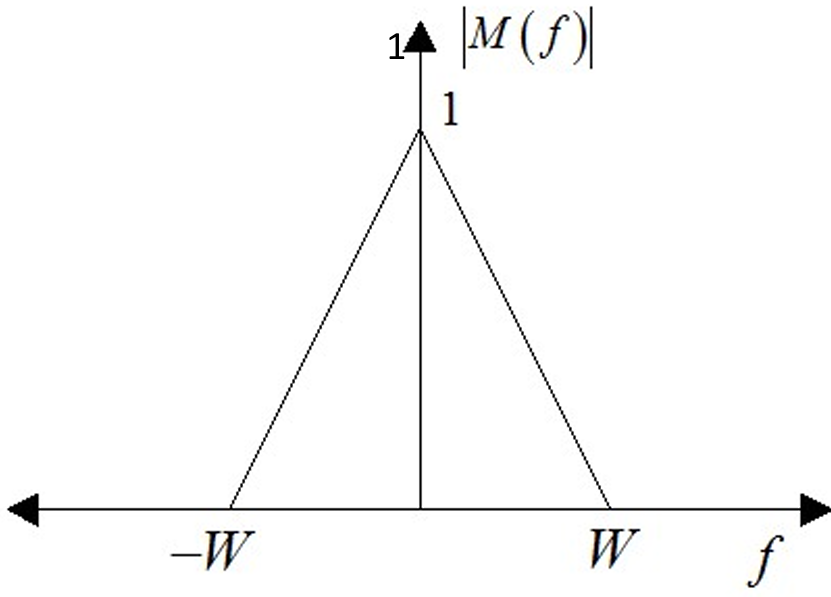
\includegraphics[width=0.6\textwidth]{fig1.png}
    \caption{Espectro de la señal de mensaje $m(t)$}
    \label{fig:1}
\end{figure}

El ancho de banda de la señal es de 1000 Hz, y es aplicada a un modulador producto con portadora $A\cos(2\pi f t)$. La señal modulada $s(t)$ es luego aplicada a un Detector Coherente como el indicado en la Fig.~\ref{fig:2} del Ejercicio 4.  

\begin{itemize}
    \item[a)] Graficar el espectro obtenido en la salida del detector para $f=500$ Hz. ¿Se recibe la señal enviada? Justifique.  
    \item[b)] Repetir para $f=10$ kHz.  
    \item[c)] Determinar la mínima frecuencia de portadora necesaria para recuperar $m(t)$ sin distorsión.  
\end{itemize}